
% POSTER EXAMPLE
%
% This is an example of a relatively sane poster. The box structure (and the
% narrative in general) is what I would expect, but it is completely
% non-mandatory; you may include whatever you want. Preferably, erase the
% existing box structure after you read it, and start from scratch.
%
% The main communication requirements for the poster that should be satisfied
% are as such:
%
% - At the defense, it should help you talk for around 10 minutes about your
%   thesis, and convince the committee that you did something interesting and
%   sufficiently complicated. Prepare pictures that explain your main results.
%
% - It should quickly communicate the main idea of your thesis to a random
%   educated by-walker. Ideally, a moderately-witted MFF graduate who has never
%   heard about your thesis before should be able to get the main "rough idea"
%   in less than 1 minute by just looking at the poster.

% modify the fontscale parameter to make everything slighly bigger or smaller.
\documentclass[portrait,fontscale=0.35,paperwidth=840mm,paperheight=1185mm]{baposter}

\usepackage[utf8]{inputenc}
\usepackage[T1]{fontenc}

% FONT CHOICES
% Posters do not need to be PDF/A; you can choose any relatable font from the
% TeX font catalogue without much risk. Sans-serif fonts are suggested for the
% posters; see https://tug.org/FontCatalogue/sansseriffonts.html
\usepackage[sfdefault]{Fira Sans}
%\usepackage[default]{droidsans}
%\usepackage[math]{iwona}
%\usepackage[defaultfam]{montserrat}
%\usepackage{cmbright}
%\usepackage{yfonts}\renewcommand{\familydefault}{\frakdefault}

\usepackage{color}
\usepackage{graphicx}
\usepackage{amssymb,amsmath}
\usepackage[export]{adjustbox} %allows using valign with \includegraphics
\usepackage{array}
\usepackage{enumitem}


\renewcommand{\arraystretch}{1.5}

\usetikzlibrary{positioning}

% A WORD ABOUT COLORS
%
% This template is prepared with a relatively neutral gray background that
% gives decent box borders (with white and darker gray), does not clash with
% many colors (except for violet-brown and other mushroomish colors, perhaps)
% and gives a lot of space for highlighting stuff.
%
% Generally, other color variations are good too; there are no strict rules on
% the colors. Good choices include:
%
% - white backgrounds and differentiation of box headers by color (see
%   headerFontColor)
%
% - various slightly tinted backgrounds (try red!10 instead of black!3)
%
% - dark backgrounds
%
% Keep in mind:
% - The normal "informative" text and figures should be DARK on LIGHT
%   background, not the other way around.
%
% - If you want a dark background, soften (darken) the box backgrounds a bit so
%   that they do not "shine" too much from the poster. Use \color{white} for
%   the heading, and switch the UK/MFF logos to white (see contents of logos/).
%
% - Do not mix too many color hues together. Most hues have their widely
%   accepted meaning (green: good result, red: problem, blue: information,
%   yellow: highlighter, brown: serious problem, violet: something really
%   weird/interesting/magic, depending on the shade).

\begin{document}

\color{black!80} % default font color
\begin{poster}{grid=false,
        eyecatcher=true,
        background=plain,
        bgColorOne=black!3, % background color
        columns=2,
        headerborder=none,
        textborder=none,
        headershape=rectangle,
        headershade=plain,
        boxshade=plain,
        boxColorOne=white,
        headershade=plain,
        headerColorOne=black!15, % box header background color
        headerFontColor=black,
    }%
    {}
    {\fontsize{13mm}{16mm}\selectfont Tower\ \ \ Defense\ \ \ Game\ \ \ with\ \ \ Procedurally\ \ \ Generated\ \ \ Content\ \ \ and\ \ \ Rogue-like\ \ \ Elements}
    {\vspace{1ex} \textbf{Vilém Gutvald} (vildagut@seznam.cz), 2024}
    {}


    %
    % LEFT COLUMN
    %

    \begin{posterbox}[column=0,name=background]{Introduction}

        \textbf{Tower defense} is a subgenre of strategy games, where the player defends against waves of attackers by building defensive towers.
        We believe that adding some mechanics from \textbf{rogue-like} games could make for a great game.
        In this thesis, we designed and inplemented such a game in Unity using C\#.
        In it, the players go through randomized procedurally generated levels with tower defense gameplay.
        They collect new towers and other blueprints from randomized offers as they go, trying to get as far as possible.
    \end{posterbox}

    \begin{posterbox}[column=0, name=goals, below=background, headerColorOne=cyan!60, boxColorOne=cyan!20]{Thesis goals}
        The main goals of the thesis were:
        \begin{itemize}[itemsep=-0.15cm,topsep=2pt]
            \item \textbf{Design} the game's mechanics and features.
            \item \textbf{Implement} a playable demo version of the game.
            \item Conduct a \textbf{playtest} to gather feedback.
        \end{itemize}
    \end{posterbox}

    \begin{posterbox}[column=0,name=design, below=goals]{Game design}

        The first goal of our thesis was to design the game.
        To do this, \textbf{we analyzed other games}, namely \textbf{\emph{Plants vs Zombies}} and \textbf{\emph{Slay the Spire}}.
        By identifying what makes them enjoyable, \textbf{we estabilished design goals} specific to our game.
        The game aims to be strategically interesting on multiple levels, it should be challenging, and it should encourage the players to explore new strategies.
        With these goals in mind, we designed the game's systems and mechanics, and created a sort of design document.

    \end{posterbox}

    \begin{posterbox}[column=0, name=game, below=design,headerColorOne=yellow!80!orange!95!black, boxColorOne=yellow!33]{Demo game features}

        Based on our design, we implemented a demo version of the game to test its core mechanics.
        A screenshot can be seen in the figure below:

        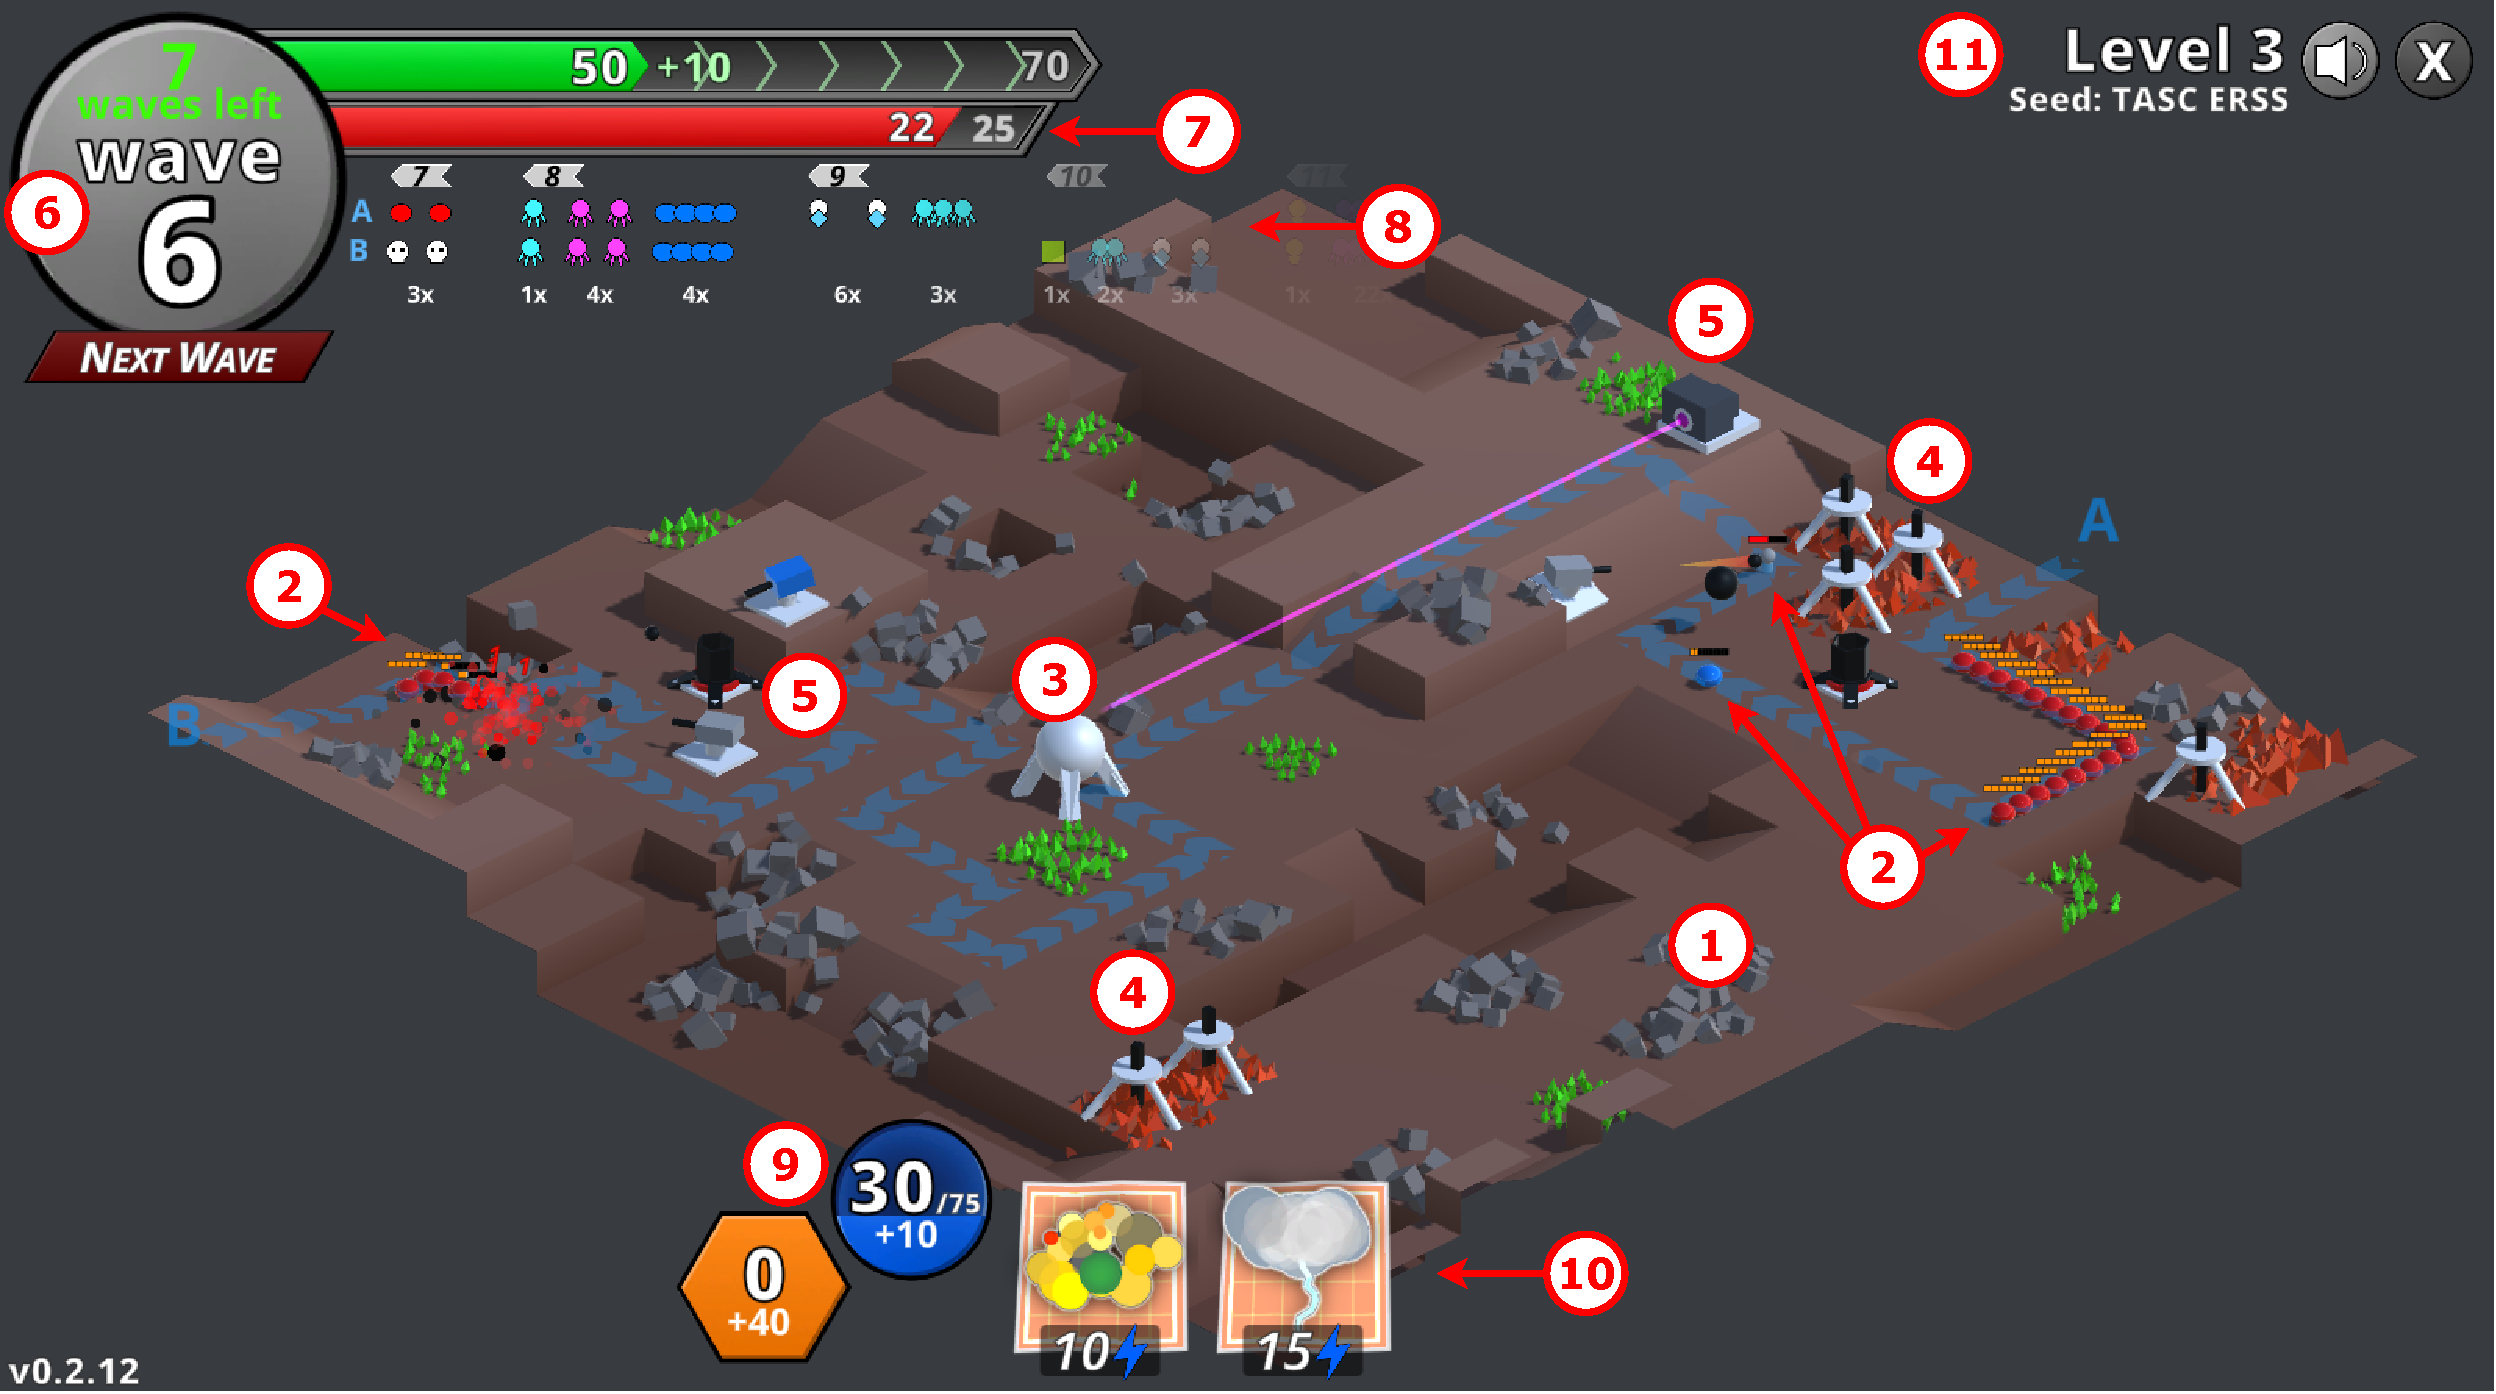
\includegraphics[width=\linewidth]{img/poster screenshot numbers.pdf}

        In the screenshot above, we can see the game world:
        \begin{enumerate}[itemsep=-0.15cm,topsep=2pt]
            \item \textbf{procedurally generated 3D terrain}, which plays an important role in the gameplay.
            \item \textbf{Attackers} coming along attacker paths, some with \textbf{special abilities}.
            \item Their target --- \textbf{the Hub}. When an attacker reaches it, the player loses some \emph{hull}.
        \end{enumerate}
        The player has placed several buildings in the world:
        \begin{enumerate}[itemsep=-0.15cm,topsep=2pt,resume]
            \item Surface drills \textbf{collecting materials}, which the player needs to build more buildings.
            \item Various \textbf{towers shooting at attackers}, each with a unique behavior and strengths.
        \end{enumerate}
        The graphical user interface communicates to the player important information:
        \begin{enumerate}[itemsep=-0.15cm,topsep=2pt,resume]
            \item The \textbf{current wave} and the number of remaining waves.
            \item Player's \textbf{\emph{hull}} (when it reaches zero, the game is over).
            \item \textbf{Preview} of the composition of \textbf{next waves}, so the player can \textbf{plan ahead}.
            \item The player's current amount of \textbf{material} (orange) and \textbf{energy} (blue).
            \item \textbf{Blueprint menu} with the blueprints the player can currently use. The ones shown here are \textbf{abilities that deal damage} to attackers within some radius when used.
            \item Current \textbf{level number} and run \textbf{seed} which completely determines this run's levels.
        \end{enumerate}

        \vspace*{2mm}
        We made a special effort to ensure everything was as clear as possible for the player.
        For example, in the figure below, we can see:
        \begin{enumerate}[itemsep=-0.15cm,topsep=2pt,resume]
            \item A \textbf{Radar} building, which increases the range of adjacent towers.
            \item And a \textbf{Gatling Gun} tower. It is currently \textbf{selected}, as denoted by the \textbf{blue highlight}. We can also see its \textbf{range} in \textbf{green}, visualising the tower's \textbf{line of sight}.
        \end{enumerate}
        On the right, we show the in-game \textbf{info panel} that shows information about the selected Gatling Gun.
        Its range statistic is \textbf{green} because it is \textbf{increased by the radar}, and some of its statistics are \textbf{red} because it needs a while to \textbf{spin up}, as per its description.
            {

                \centering
                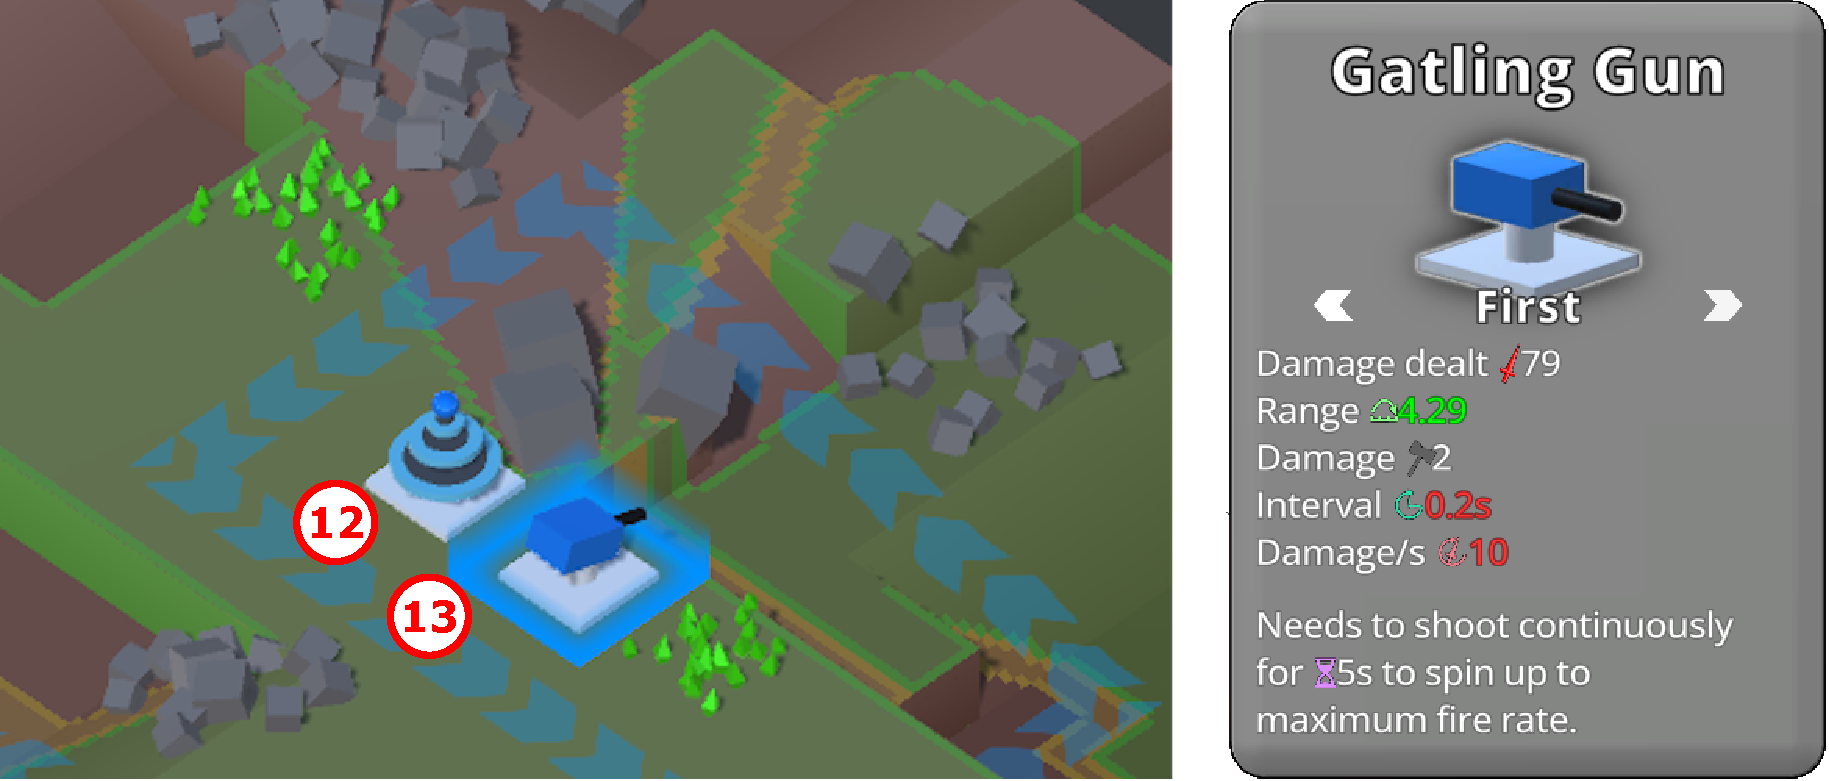
\includegraphics[width=0.6\linewidth]{img/poster tower numbers.pdf}

            }

    \end{posterbox}

    %
    % FOOTER
    %

    \begin{posterbox}[column=0, span=2, name=footer, below=game,
            textborder=none, headerborder=none, boxheaderheight=0pt,
            boxColorOne=black!15]{}
        \begin{tabular}{m{10.6cm}m{9.8cm}m{3cm}m{3cm}}
            
\includegraphics[trim={0.4cm 1.2cm 0.9cm 1.2cm}, clip, width=\linewidth]{img/logotyp_fakulty4.pdf}
             &
            Supervisor:\ \ Mgr. Pavel Ježek, Ph.D. \newline
            Department of Distributed and Dependable Systems
             &
            \centering
            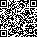
\includegraphics[width=1.3cm]{img/game QR.png}


            Game (Windows)
             &
            \centering
            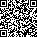
\includegraphics[width=1.3cm]{img/thesis QR.png}


            Thesis
        \end{tabular}
    \end{posterbox}


    %
    % RIGHT COLUMN
    %
    % It is usually best to fill most of the poster with your results and
    % conclusions. Again, use simple annotated pictures wherever possible. Plots
    % with measurements are perfect, tables are also good.
    %

    \begin{posterbox}[column=1,name=levels]{Procedurally generating Levels}

        The levels and blueprint rewards in each run are randomized.
        However, this randomness is \textbf{fully determined by the run seed}.
        The image below shows a simplified overview of the level generation.
        Based on the run seed, we generate the level seed and the level parameters.
        We have set many requirements for the generated worlds, and to fulfill them, we had to come up with sophisticated algorithms.

        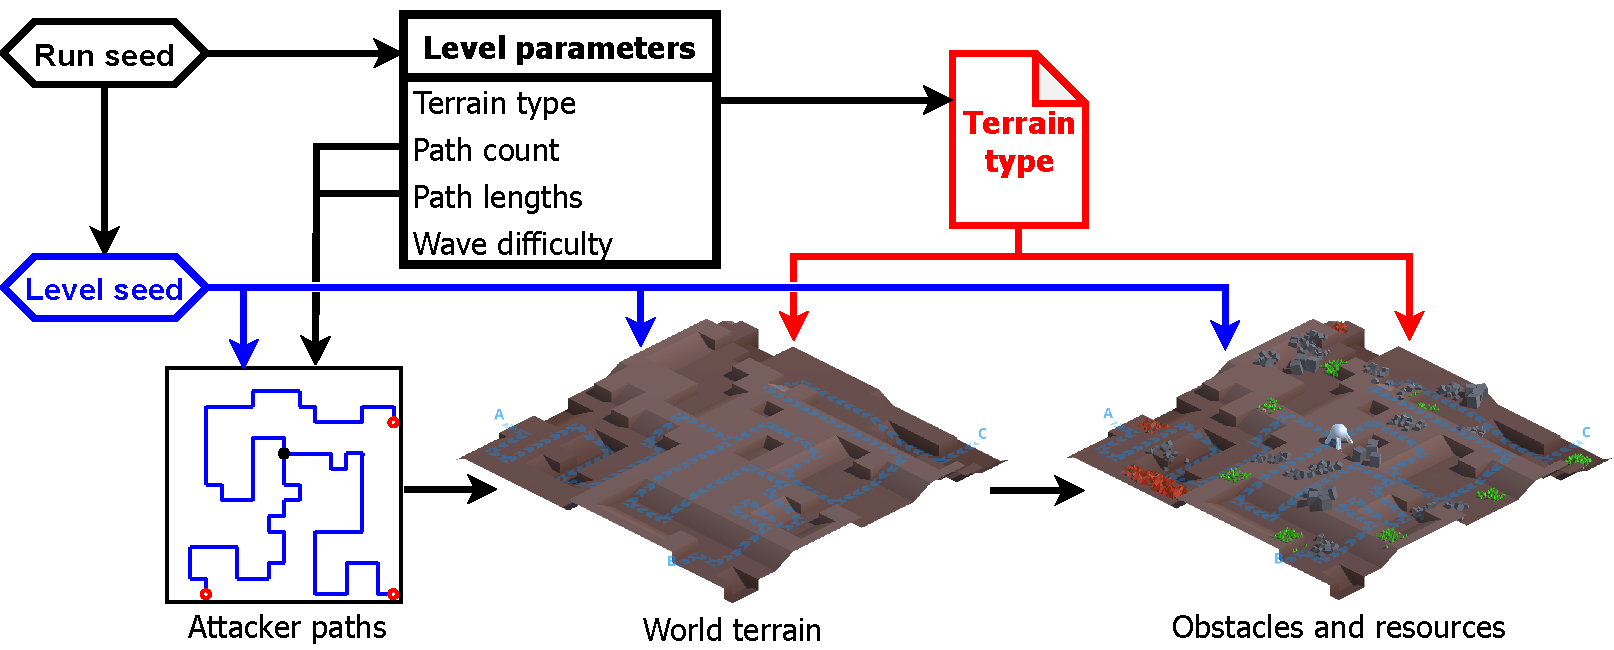
\includegraphics[width=\linewidth]{img/world PG diagram.pdf}

        First, we generate the \textbf{attacker paths} based on level parameters such as the path lengths.
        This is done in several steps, for which we developed custom algorithms.
        For example, we adapted \textbf{simulated annealing} to use it to optimize the path shapes.
        This lets us create complex path networks that feel \textbf{unique but fair}.

        Then the \textbf{3D terrain} is generated.
        To allow different levels to look and feel more different, the terrain components are specified using a custom \textbf{terrain type} file.
        To generate the terrain, we use our custom implementation of \textbf{wave function collapse}.
        This lets us generate randomized terrain from the \textbf{components we specify} that also respects many requirements, for example that paths cannot go through a cliff.

        Finally, we distribute \textbf{obstacles and resources} on the generated world, which are also customizable in the terrain type file.
        To make them \textbf{look natural}, we procedurally generate their appearance by randomly \textbf{scattering models} on the world surface.

    \end{posterbox}

    \begin{posterbox}[column=1,name=waves,below=levels]{Procedurally generating Attacker waves}

        In each level, the player has to defend against several waves of attackers.
        Each wave is procedurally generated from a catalog of attackers, such that it has the desired difficulty.
        Since there is no algorithm which satisfies our requirements, we use a \textbf{custom algorithm}.
        To create it, we first had to develop a way to \textbf{quantify wave difficulty} that is accurate enough to generate fair waves.
        Below is an example of different waves generated with the same given desired difficulty and attacker catalog:

        \centering
        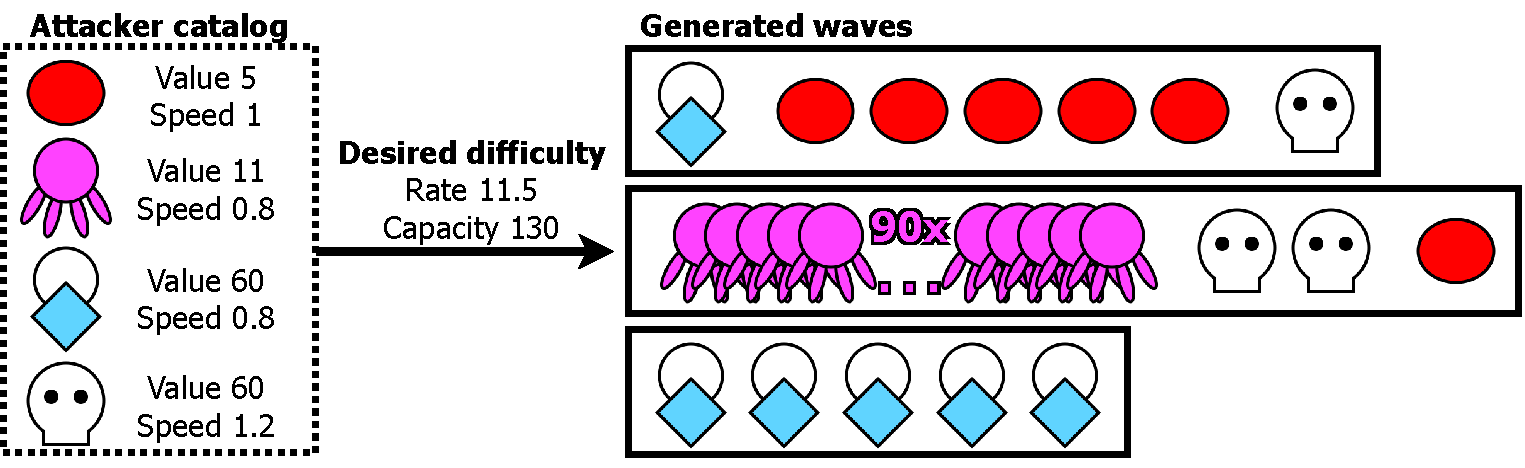
\includegraphics[width=0.7\linewidth]{img/wave generation.pdf}

    \end{posterbox}

    \begin{posterbox}[column=1,name=tutorial, below=waves]{In-game Tutorial}

        The game includes an \textbf{interactive tutorial} that guides players and explains the main mechanics. This tutorial proved \textbf{very effective}, allowing players to play and learn more without external help. One step of the tutorial is shown in the image below.

        \centering
        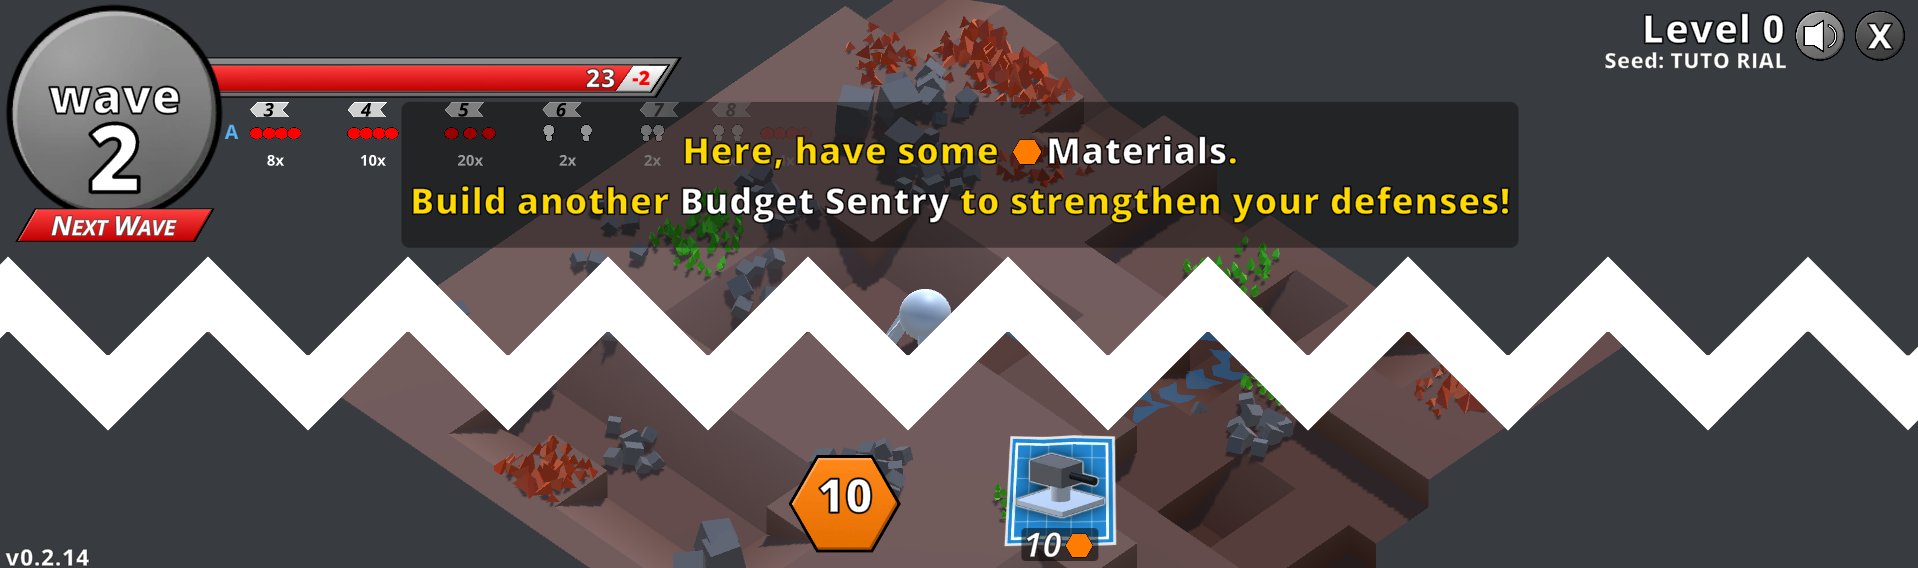
\includegraphics[width=\linewidth]{img/tutorial-cut.png}

    \end{posterbox}

    \begin{posterbox}[column=1, name=playtest, below=tutorial, headerColorOne=green!50!yellow, boxColorOne=green!10]{Playtest results}
        Finally, we conducted a playtest and gathered feedback from \textbf{11 players}.
        During the playtesting, we fixed few bugs the players found, and we tweaked the game balance to make it more fun.
        The feedback showed that the game's systems were designed well, and overall, the \textbf{players enjoyed the game}.
        It has \textbf{a lot of strategic depth} even as a demo version.
        However, the game also has several issues.
        Some are addressed by the features we planned for later, others will require some systems to be redesigned.
    \end{posterbox}

    \begin{posterbox}[column=1, name=conclusion, below=playtest, bottomaligned=game]{Conclusion}
        In conclusion, \textbf{we achieved our goals} and developed an \textbf{engaging game} with great \mbox{potential}.
        The algorithms we developed effectively address the problems they were designed to solve.
        However, there is still more work to be done, including implementing planned features, fixing issues, and adding more content.
    \end{posterbox}

\end{poster}
\end{document}
